 \documentclass[border=5pt]{standalone}
     \usepackage[svgnames]{xcolor}
   
    \usepackage{tikz}
    \usetikzlibrary{matrix,decorations.pathreplacing, calc, positioning,fit}
    \usepackage{amsmath}
    \usepackage{mathtools}
 
    \begin{document}

    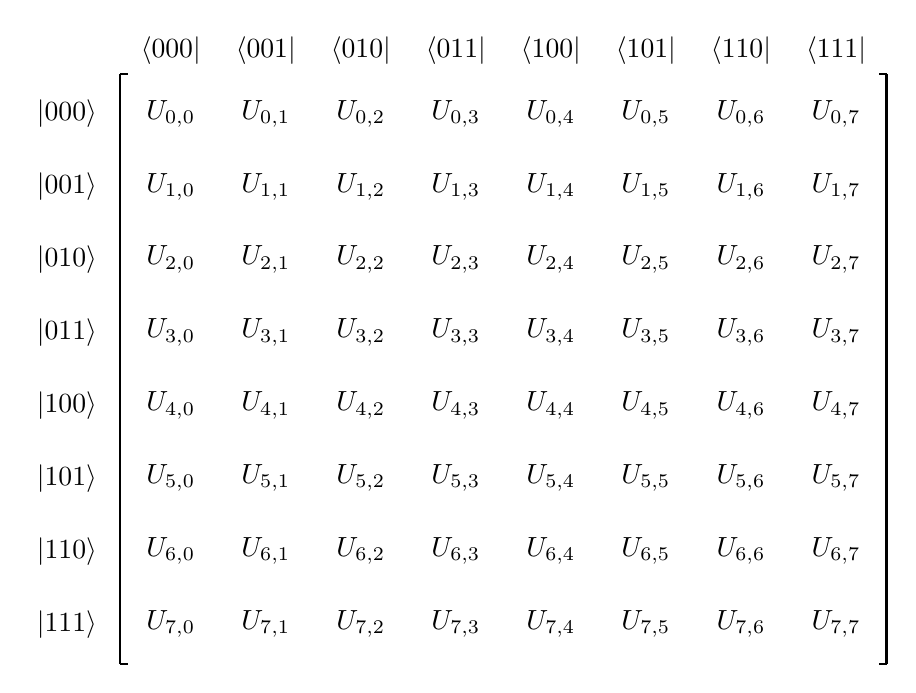
\begin{tikzpicture}[>=stealth,thick,baseline]
    \matrix [matrix of math nodes, row sep=1em, column sep=1em,](A){ 
    U_{0,0}&U_{0,1}&U_{0,2}&U_{0,3}&U_{0,4}&U_{0,5}&U_{0,6}&U_{0,7}\\
    U_{1,0}&U_{1,1}&U_{1,2}&U_{1,3}&U_{1,4}&U_{1,5}&U_{1,6}&U_{1,7}\\
    U_{2,0}&U_{2,1}&U_{2,2}&U_{2,3}&U_{2,4}&U_{2,5}&U_{2,6}&U_{2,7}\\
    U_{3,0}&U_{3,1}&U_{3,2}&U_{3,3}&U_{3,4}&U_{3,5}&U_{3,6}&U_{3,7}\\
    U_{4,0}&U_{4,1}&U_{4,2}&U_{4,3}&U_{4,4}&U_{4,5}&U_{4,6}&U_{4,7}\\
    U_{5,0}&U_{5,1}&U_{5,2}&U_{5,3}&U_{5,4}&U_{5,5}&U_{5,6}&U_{5,7}\\
    U_{6,0}&U_{6,1}&U_{6,2}&U_{6,3}&U_{6,4}&U_{6,5}&U_{6,6}&U_{6,7}\\
    U_{7,0}&U_{7,1}&U_{7,2}&U_{7,3}&U_{7,4}&U_{7,5}&U_{7,6}&U_{7,7}\\
    };

	\draw[]  ($(A-1-1.north west) + (-0.2,+0.2)$) -- ($(A-8-1.south west) + (-0.2,-0.2)$);
	\draw[]  ($(A-1-1.north west) + (-0.2,+0.2)$) -- ++(0.1,0);
	\draw[]  ($(A-8-1.south west) + (-0.2,-0.2)$) -- ++(0.1,0); 	

	\draw[]  ($(A-1-8.north east) + (+0.2,+0.2)$) -- ($(A-8-8.south east) + (+0.2,-0.2)$);
	\draw[]  ($(A-1-8.north east) + (+0.2,+0.2)$) -- ++(-0.1,0);
	\draw[]  ($(A-8-8.south east) + (+0.2,-0.2)$) -- ++(-0.1,0); 	

%
%	\draw[thin]  ($(A-1-1.north west) + (-0.1,+0.1)$) -- ($(A-4-1.south west) + (-0.1,-0.1)$);
%	\draw[thin]  ($(A-1-1.north west) + (-0.1,+0.1)$) -- ++(0.1,0);
%	\draw[thin]  ($(A-4-1.south west) + (-0.1,-0.1)$) -- ++(0.1,0);
%
%	\draw[thin]  ($(A-5-1.north west) + (-0.1,+0.1)$) -- ($(A-8-1.south west) + (-0.1,-0.1)$);
%	\draw[thin]  ($(A-5-1.north west) + (-0.1,+0.1)$) -- ++(0.1,0);
%	\draw[thin]  ($(A-8-1.south west) + (-0.1,-0.1)$) -- ++(0.1,0);
%
%	\draw[thin]  ($(A-1-5.north west) + (-0.1,+0.1)$) -- ($(A-4-5.south west) + (-0.1,-0.1)$);
%	\draw[thin]  ($(A-1-5.north west) + (-0.1,+0.1)$) -- ++(0.1,0);
%	\draw[thin]  ($(A-4-5.south west) + (-0.1,-0.1)$) -- ++(0.1,0);
%
%	\draw[thin]  ($(A-5-5.north west) + (-0.1,+0.1)$) -- ($(A-8-5.south west) + (-0.1,-0.1)$);
%	\draw[thin]  ($(A-5-5.north west) + (-0.1,+0.1)$) -- ++(0.1,0);
%	\draw[thin]  ($(A-8-5.south west) + (-0.1,-0.1)$) -- ++(0.1,0);
%
%
%	\draw[thin]  ($(A-1-4.north east) + (+0.1,+0.1)$) -- ($(A-4-4.south east) + (+0.1,-0.1)$);
%	\draw[thin]  ($(A-1-4.north east) + (+0.1,+0.1)$) -- ++(-0.1,0);
%	\draw[thin]  ($(A-4-4.south east) + (+0.1,-0.1)$) -- ++(-0.1,0);
%
%	\draw[thin]  ($(A-5-4.north east) + (+0.1,+0.1)$) -- ($(A-8-4.south east) + (+0.1,-0.1)$);
%	\draw[thin]  ($(A-5-4.north east) + (+0.1,+0.1)$) -- ++(-0.1,0);
%	\draw[thin]  ($(A-8-4.south east) + (+0.1,-0.1)$) -- ++(-0.1,0);
%
%
%	\draw[thin]  ($(A-1-8.north east) + (+0.1,+0.1)$) -- ($(A-4-8.south east) + (+0.1,-0.1)$);
%	\draw[thin]  ($(A-1-8.north east) + (+0.1,+0.1)$) -- ++(-0.1,0);
%	\draw[thin]  ($(A-4-8.south east) + (+0.1,-0.1)$) -- ++(-0.1,0);
%
%	\draw[thin]  ($(A-5-8.north east) + (+0.1,+0.1)$) -- ($(A-8-8.south east) + (+0.1,-0.1)$);
%	\draw[thin]  ($(A-5-8.north east) + (+0.1,+0.1)$) -- ++(-0.1,0);
%	\draw[thin]  ($(A-8-8.south east) + (+0.1,-0.1)$) -- ++(-0.1,0);
%
%
%	\draw[ultra thin]  (A-1-1.north west) -- ++(0.1,0);
%	\draw[ultra thin]  (A-1-1.north west) -- 
%	                   (A-2-1.south west);
%	\draw[ultra thin]  (A-2-1.south west) -- ++(0.1,0);	
%	
%	\draw[ultra thin]  (A-1-2.north east) -- ++(-0.1,0);
%	\draw[ultra thin]  (A-1-2.north east) -- 
%	                   (A-2-2.south east);
%	\draw[ultra thin]  (A-2-2.south east) -- ++(-0.1,0);	
%	
%	\draw[ultra thin]  (A-3-1.north west) -- ++(0.1,0);
%	\draw[ultra thin]  (A-3-1.north west) -- 
%	                   (A-4-1.south west);
%	\draw[ultra thin]  (A-4-1.south west) -- ++(0.1,0);	
%	
%	\draw[ultra thin]  (A-3-2.north east) -- ++(-0.1,0);
%	\draw[ultra thin]  (A-3-2.north east) -- 
%	                   (A-4-2.south east);
%	\draw[ultra thin]  (A-4-2.south east) -- ++(-0.1,0);	
%	
%	\draw[ultra thin]  (A-5-1.north west) -- ++(0.1,0);
%	\draw[ultra thin]  (A-5-1.north west) -- 
%	                   (A-6-1.south west);
%	\draw[ultra thin]  (A-6-1.south west) -- ++(0.1,0);	
%	
%	\draw[ultra thin]  (A-5-2.north east) -- ++(-0.1,0);
%	\draw[ultra thin]  (A-5-2.north east) -- 
%	                   (A-6-2.south east);
%	\draw[ultra thin]  (A-6-2.south east) -- ++(-0.1,0);	
%	
%	\draw[ultra thin]  (A-7-1.north west) -- ++(0.1,0);
%	\draw[ultra thin]  (A-7-1.north west) -- 
%	                   (A-8-1.south west);
%	\draw[ultra thin]  (A-8-1.south west) -- ++(0.1,0);	
%	
%	\draw[ultra thin]  (A-7-2.north east) -- ++(-0.1,0);
%	\draw[ultra thin]  (A-7-2.north east) -- 
%	                   (A-8-2.south east);
%	\draw[ultra thin]  (A-8-2.south east) -- ++(-0.1,0);	
%
%
%	\draw[ultra thin]  (A-1-3.north west) -- ++(0.1,0);
%	\draw[ultra thin]  (A-1-3.north west) -- 
%	                   (A-2-3.south west);
%	\draw[ultra thin]  (A-2-3.south west) -- ++(0.1,0);	
%	
%	\draw[ultra thin]  (A-1-4.north east) -- ++(-0.1,0);
%	\draw[ultra thin]  (A-1-4.north east) -- 
%	                   (A-2-4.south east);
%	\draw[ultra thin]  (A-2-4.south east) -- ++(-0.1,0);	
%	
%	\draw[ultra thin]  (A-3-3.north west) -- ++(0.1,0);
%	\draw[ultra thin]  (A-3-3.north west) -- 
%	                   (A-4-3.south west);
%	\draw[ultra thin]  (A-4-3.south west) -- ++(0.1,0);	
%	
%	\draw[ultra thin]  (A-3-4.north east) -- ++(-0.1,0);
%	\draw[ultra thin]  (A-3-4.north east) -- 
%	                   (A-4-4.south east);
%	\draw[ultra thin]  (A-4-4.south east) -- ++(-0.1,0);	
%	
%	\draw[ultra thin]  (A-5-3.north west) -- ++(0.1,0);
%	\draw[ultra thin]  (A-5-3.north west) -- 
%	                   (A-6-3.south west);
%	\draw[ultra thin]  (A-6-3.south west) -- ++(0.1,0);	
%	
%	\draw[ultra thin]  (A-5-4.north east) -- ++(-0.1,0);
%	\draw[ultra thin]  (A-5-4.north east) -- 
%	                   (A-6-4.south east);
%	\draw[ultra thin]  (A-6-4.south east) -- ++(-0.1,0);	
%	
%	\draw[ultra thin]  (A-7-3.north west) -- ++(0.1,0);
%	\draw[ultra thin]  (A-7-3.north west) -- 
%	                   (A-8-3.south west);
%	\draw[ultra thin]  (A-8-3.south west) -- ++(0.1,0);	
%	
%	\draw[ultra thin]  (A-7-4.north east) -- ++(-0.1,0);
%	\draw[ultra thin]  (A-7-4.north east) -- 
%	                   (A-8-4.south east);
%	\draw[ultra thin]  (A-8-4.south east) -- ++(-0.1,0);	
%	
%
%	\draw[ultra thin]  (A-1-3.north west) -- ++(0.1,0);
%	\draw[ultra thin]  (A-1-3.north west) -- 
%	                   (A-2-3.south west);
%	\draw[ultra thin]  (A-2-3.south west) -- ++(0.1,0);	
%	
%	\draw[ultra thin]  (A-1-4.north east) -- ++(-0.1,0);
%	\draw[ultra thin]  (A-1-4.north east) -- 
%	                   (A-2-4.south east);
%	\draw[ultra thin]  (A-2-4.south east) -- ++(-0.1,0);	
%	
%	\draw[ultra thin]  (A-3-3.north west) -- ++(0.1,0);
%	\draw[ultra thin]  (A-3-3.north west) -- 
%	                   (A-4-3.south west);
%	\draw[ultra thin]  (A-4-3.south west) -- ++(0.1,0);	
%	
%	\draw[ultra thin]  (A-3-4.north east) -- ++(-0.1,0);
%	\draw[ultra thin]  (A-3-4.north east) -- 
%	                   (A-4-4.south east);
%	\draw[ultra thin]  (A-4-4.south east) -- ++(-0.1,0);	
%	
%	\draw[ultra thin]  (A-5-3.north west) -- ++(0.1,0);
%	\draw[ultra thin]  (A-5-3.north west) -- 
%	                   (A-6-3.south west);
%	\draw[ultra thin]  (A-6-3.south west) -- ++(0.1,0);	
%	
%	\draw[ultra thin]  (A-5-4.north east) -- ++(-0.1,0);
%	\draw[ultra thin]  (A-5-4.north east) -- 
%	                   (A-6-4.south east);
%	\draw[ultra thin]  (A-6-4.south east) -- ++(-0.1,0);	
%	
%	\draw[ultra thin]  (A-7-3.north west) -- ++(0.1,0);
%	\draw[ultra thin]  (A-7-3.north west) -- 
%	                   (A-8-3.south west);
%	\draw[ultra thin]  (A-8-3.south west) -- ++(0.1,0);	
%	
%	\draw[ultra thin]  (A-7-4.north east) -- ++(-0.1,0);
%	\draw[ultra thin]  (A-7-4.north east) -- 
%	                   (A-8-4.south east);
%	\draw[ultra thin]  (A-8-4.south east) -- ++(-0.1,0);	
%	
%	
%
%	\draw[ultra thin]  (A-1-5.north west) -- ++(0.1,0);
%	\draw[ultra thin]  (A-1-5.north west) -- 
%	                   (A-2-5.south west);
%	\draw[ultra thin]  (A-2-5.south west) -- ++(0.1,0);	
%	
%	\draw[ultra thin]  (A-1-6.north east) -- ++(-0.1,0);
%	\draw[ultra thin]  (A-1-6.north east) -- 
%	                   (A-2-6.south east);
%	\draw[ultra thin]  (A-2-6.south east) -- ++(-0.1,0);	
%	
%	\draw[ultra thin]  (A-3-5.north west) -- ++(0.1,0);
%	\draw[ultra thin]  (A-3-5.north west) -- 
%	                   (A-4-5.south west);
%	\draw[ultra thin]  (A-4-5.south west) -- ++(0.1,0);	
%	
%	\draw[ultra thin]  (A-3-6.north east) -- ++(-0.1,0);
%	\draw[ultra thin]  (A-3-6.north east) -- 
%	                   (A-4-6.south east);
%	\draw[ultra thin]  (A-4-6.south east) -- ++(-0.1,0);	
%	
%	\draw[ultra thin]  (A-5-5.north west) -- ++(0.1,0);
%	\draw[ultra thin]  (A-5-5.north west) -- 
%	                   (A-6-5.south west);
%	\draw[ultra thin]  (A-6-5.south west) -- ++(0.1,0);	
%	
%	\draw[ultra thin]  (A-5-6.north east) -- ++(-0.1,0);
%	\draw[ultra thin]  (A-5-6.north east) -- 
%	                   (A-6-6.south east);
%	\draw[ultra thin]  (A-6-6.south east) -- ++(-0.1,0);	
%	
%	\draw[ultra thin]  (A-7-5.north west) -- ++(0.1,0);
%	\draw[ultra thin]  (A-7-5.north west) -- 
%	                   (A-8-5.south west);
%	\draw[ultra thin]  (A-8-5.south west) -- ++(0.1,0);	
%	
%	\draw[ultra thin]  (A-7-6.north east) -- ++(-0.1,0);
%	\draw[ultra thin]  (A-7-6.north east) -- 
%	                   (A-8-6.south east);
%	\draw[ultra thin]  (A-8-6.south east) -- ++(-0.1,0);	
%		
%	
%	
%	
%	
%	\draw[ultra thin]  (A-1-7.north west) -- ++(0.1,0);
%	\draw[ultra thin]  (A-1-7.north west) -- 
%	                   (A-2-7.south west);
%	\draw[ultra thin]  (A-2-7.south west) -- ++(0.1,0);	
%	
%	\draw[ultra thin]  (A-1-8.north east) -- ++(-0.1,0);
%	\draw[ultra thin]  (A-1-8.north east) -- 
%	                   (A-2-8.south east);
%	\draw[ultra thin]  (A-2-8.south east) -- ++(-0.1,0);	
%	
%	\draw[ultra thin]  (A-3-7.north west) -- ++(0.1,0);
%	\draw[ultra thin]  (A-3-7.north west) -- 
%	                   (A-4-7.south west);
%	\draw[ultra thin]  (A-4-7.south west) -- ++(0.1,0);	
%	
%	\draw[ultra thin]  (A-3-8.north east) -- ++(-0.1,0);
%	\draw[ultra thin]  (A-3-8.north east) -- 
%	                   (A-4-8.south east);
%	\draw[ultra thin]  (A-4-8.south east) -- ++(-0.1,0);	
%	
%	\draw[ultra thin]  (A-5-7.north west) -- ++(0.1,0);
%	\draw[ultra thin]  (A-5-7.north west) -- 
%	                   (A-6-7.south west);
%	\draw[ultra thin]  (A-6-7.south west) -- ++(0.1,0);	
%	
%	\draw[ultra thin]  (A-5-8.north east) -- ++(-0.1,0);
%	\draw[ultra thin]  (A-5-8.north east) -- 
%	                   (A-6-8.south east);
%	\draw[ultra thin]  (A-6-8.south east) -- ++(-0.1,0);	
%	
%	\draw[ultra thin]  (A-7-7.north west) -- ++(0.1,0);
%	\draw[ultra thin]  (A-7-7.north west) -- 
%	                   (A-8-7.south west);
%	\draw[ultra thin]  (A-8-7.south west) -- ++(0.1,0);	
%	
%	\draw[ultra thin]  (A-7-8.north east) -- ++(-0.1,0);
%	\draw[ultra thin]  (A-7-8.north east) -- 
%	                   (A-8-8.south east);
%	\draw[ultra thin]  (A-8-8.south east) -- ++(-0.1,0);	
%	
%	
%   \node[
%     fit=(A-1-4)(A-1-5),
%     inner xsep=5pt,inner ysep=20pt,
%     label=above: in-side   
%     ](K01) {};
%
%   \node[
%     fit=(A-4-1)(A-5-1),
%     inner xsep=50pt,inner ysep=-5pt,
%     label={[rotate=90]left:out-side}
%     ](K01) {};




   \node[
     fit=(A-1-1)(A-1-1),
     inner xsep=5pt,inner ysep=5pt,
     label=above: $\langle 000|$
    ](K00) {};

   \node[
     fit=(A-1-2)(A-1-2),
     inner xsep=5pt,inner ysep=5pt,
     label=above: $\langle 001|$
    ](K01) {};


   \node[
     fit=(A-1-3)(A-1-3),
     inner xsep=5pt,inner ysep=5pt,
     label=above: $\langle 010|$
    ](K10) {};

   \node[
     fit=(A-1-4)(A-1-4),
     inner xsep=5pt,inner ysep=5pt,
     label=above: $\langle 011|$
    ](K10) {};


   \node[
     fit=(A-1-5)(A-1-5),
     inner xsep=5pt,inner ysep=5pt,
     label=above: $\langle 100|$
    ](K00) {};

   \node[
     fit=(A-1-6)(A-1-6),
     inner xsep=5pt,inner ysep=5pt,
     label=above: $\langle 101|$
    ](K01) {};

   \node[
     fit=(A-1-7)(A-1-7),
     inner xsep=5pt,inner ysep=5pt,
     label=above: $\langle 110|$
    ](K10) {};
   \node[
     fit=(A-1-8)(A-1-8),
     inner xsep=5pt,inner ysep=5pt,
     label=above: $\langle 111|$
    ](K11) {};


   \node[
     fit=(A-1-1)(A-1-1),
     inner xsep=10pt,inner ysep=5pt,
     label=left: $|000\rangle$
    ](K00) {};

   \node[
     fit=(A-2-1)(A-2-1),
     inner xsep=10pt,inner ysep=5pt,
     label=left: $|001\rangle$
    ](K01) {};


   \node[
     fit=(A-3-1)(A-3-1),
     inner xsep=10pt,inner ysep=5pt,
     label=left: $|010\rangle$
    ](K10) {};


   \node[
     fit=(A-4-1)(A-4-1),
     inner xsep=10pt,inner ysep=5pt,
     label=left: $|011\rangle$
    ](K11) {};


   \node[
     fit=(A-5-1)(A-5-1),
     inner xsep=10pt,inner ysep=5pt,
     label=left: $|100\rangle$
    ](K00) {};

   \node[
     fit=(A-6-1)(A-6-1),
     inner xsep=10pt,inner ysep=5pt,
     label=left: $|101\rangle$
    ](K01) {};


   \node[
     fit=(A-7-1)(A-7-1),
     inner xsep=10pt,inner ysep=5pt,
     label=left: $|110\rangle$
    ](K10) {};


   \node[
     fit=(A-8-1)(A-8-1),
     inner xsep=10pt,inner ysep=5pt,
     label=left: $|111\rangle$
    ](K11) {};


    \end{tikzpicture}

\end{document}
    
    
    